% !TEX root = morphkasten.tex

\section{Containererkennung (grob)}


%##############
\subsection{Distanz und Farbsensor}

\begin{figure} [hbp]
	\centering
	\includegraphics[width=0.5\textwidth]{fig/Containererkennung_2.png}
	\caption{Beispielhafte Containererkennung mit Distanz- und Farbsensoren}
\end{figure}

\begin{table}[h]
\begin{tabular}{p{0.5\textwidth} | p{0.5\textwidth}}


 \textbf{Vorteile} & \textbf{Nachteile} \\ \hline
	 
\begin{itemize}
\item Präzise Erkennung des Containers (wahrscheinlich)
\item Mehrfachverwendung mit anderen Anwendungen denkbar
\item Kostengünstig
\end{itemize}

 
 &
 
\begin{itemize}
\item Unbekannte Präzision
\item Je nach Sensor Störanfälligkeit
\item Zusatzhardware(Farb und Distanzsensor) und Verkabelung nötig
\end{itemize}

\end{tabular}
\end{table}

\begin{table}[h]
\begin{tabular}{p{0.5\textwidth}p{0.5\textwidth}}


 \textbf{Risiken} & \\ \hline
	 
\begin{itemize}
\item Die Sensoren sind zu ungenau
\item Die Sensoren werden gestört
\item Das Fahrzeug kann nicht schnell genug anhalten
\end{itemize}
&
\begin{itemize}
\item Die Farbe kann auf Distanz nicht erkannt werden
\item Die Sensoren können zwischen Container und Sonstigem nicht unterscheiden
\item Die Container können bei der volle Geschwindigkeit nicht erkannt werden
\end{itemize}

 
\end{tabular}
\end{table}

\pagebreak


%##############
\subsection{Bilderkennung}
\begin{figure}[h!]%Position festigen
\centering
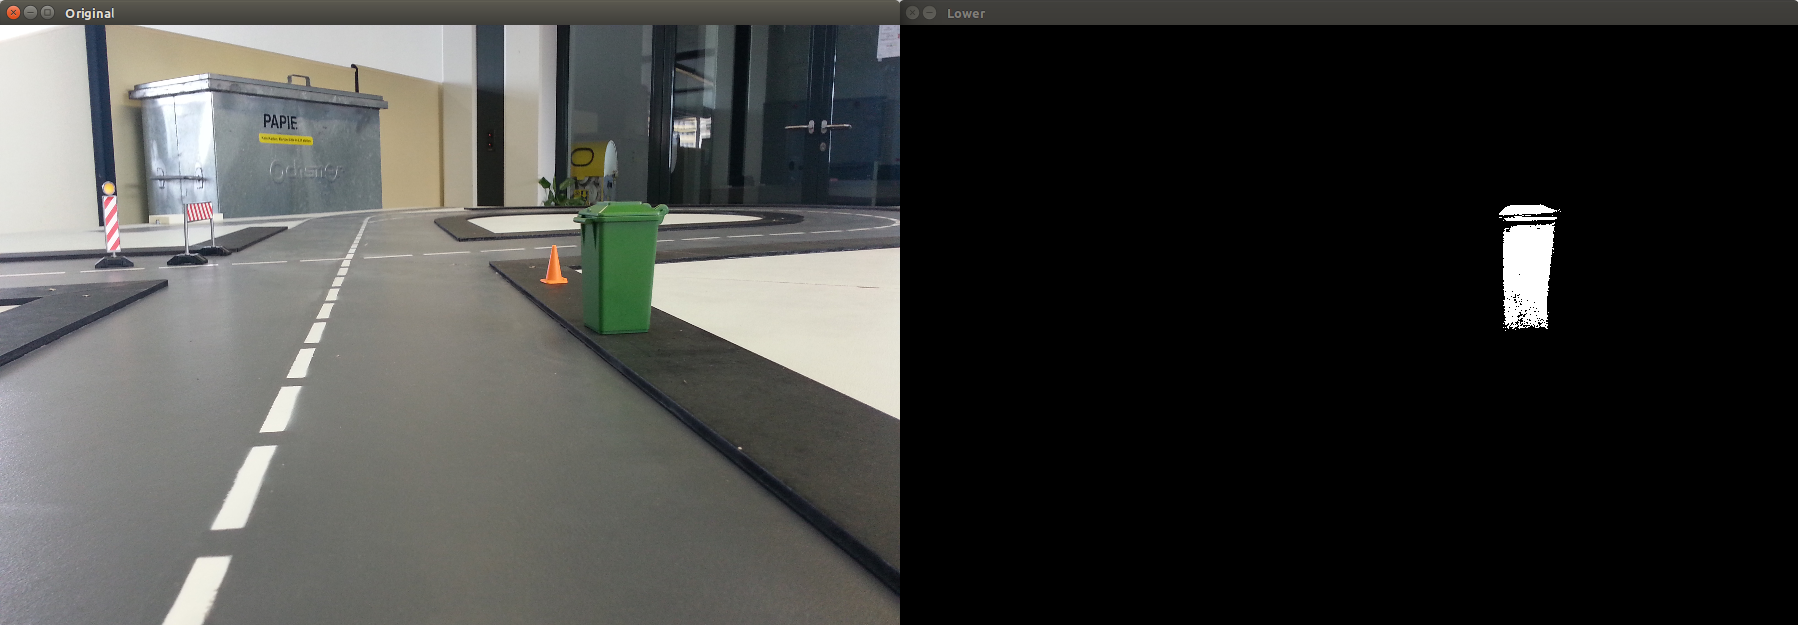
\includegraphics[width=0.7\textwidth]{fig/containererkennung_grob_bilderkennung.png}
\caption{Bilderkennung Container}
\label{fig:Bilderkennung Container}
\end{figure}

\begin{table}[h]
\begin{tabular}{p{0.5\textwidth} | p{0.5\textwidth}}


\textbf{Vorteile} & \textbf{Nachteile} \\ \hline
	 
\begin{itemize}
\item bei grösserer Distanz zu Container schon erkennbar
\item Containererkennung durch Form- und/oder Farberkennung
\end{itemize}

 
 &
 
\begin{itemize}
\item Algorithmus nötig
\item rechenintensiv
\end{itemize}

\end{tabular}
\end{table}

\begin{table}[h]
\begin{tabular}{p{0.5\textwidth}p{0.5\textwidth}}

\textbf{Risiken} & \\ \hline
	 
\begin{itemize}
\item bei verschiedene Lichtverhätlnissen variieren die Farben
\item Container kann zum Teil von anderen Gegeständen verdeckt sein
\end{itemize}

 
\end{tabular}
\end{table}

\pagebreak